
\section{Experiments}

% \begin{figure}
% 	\centering
% 	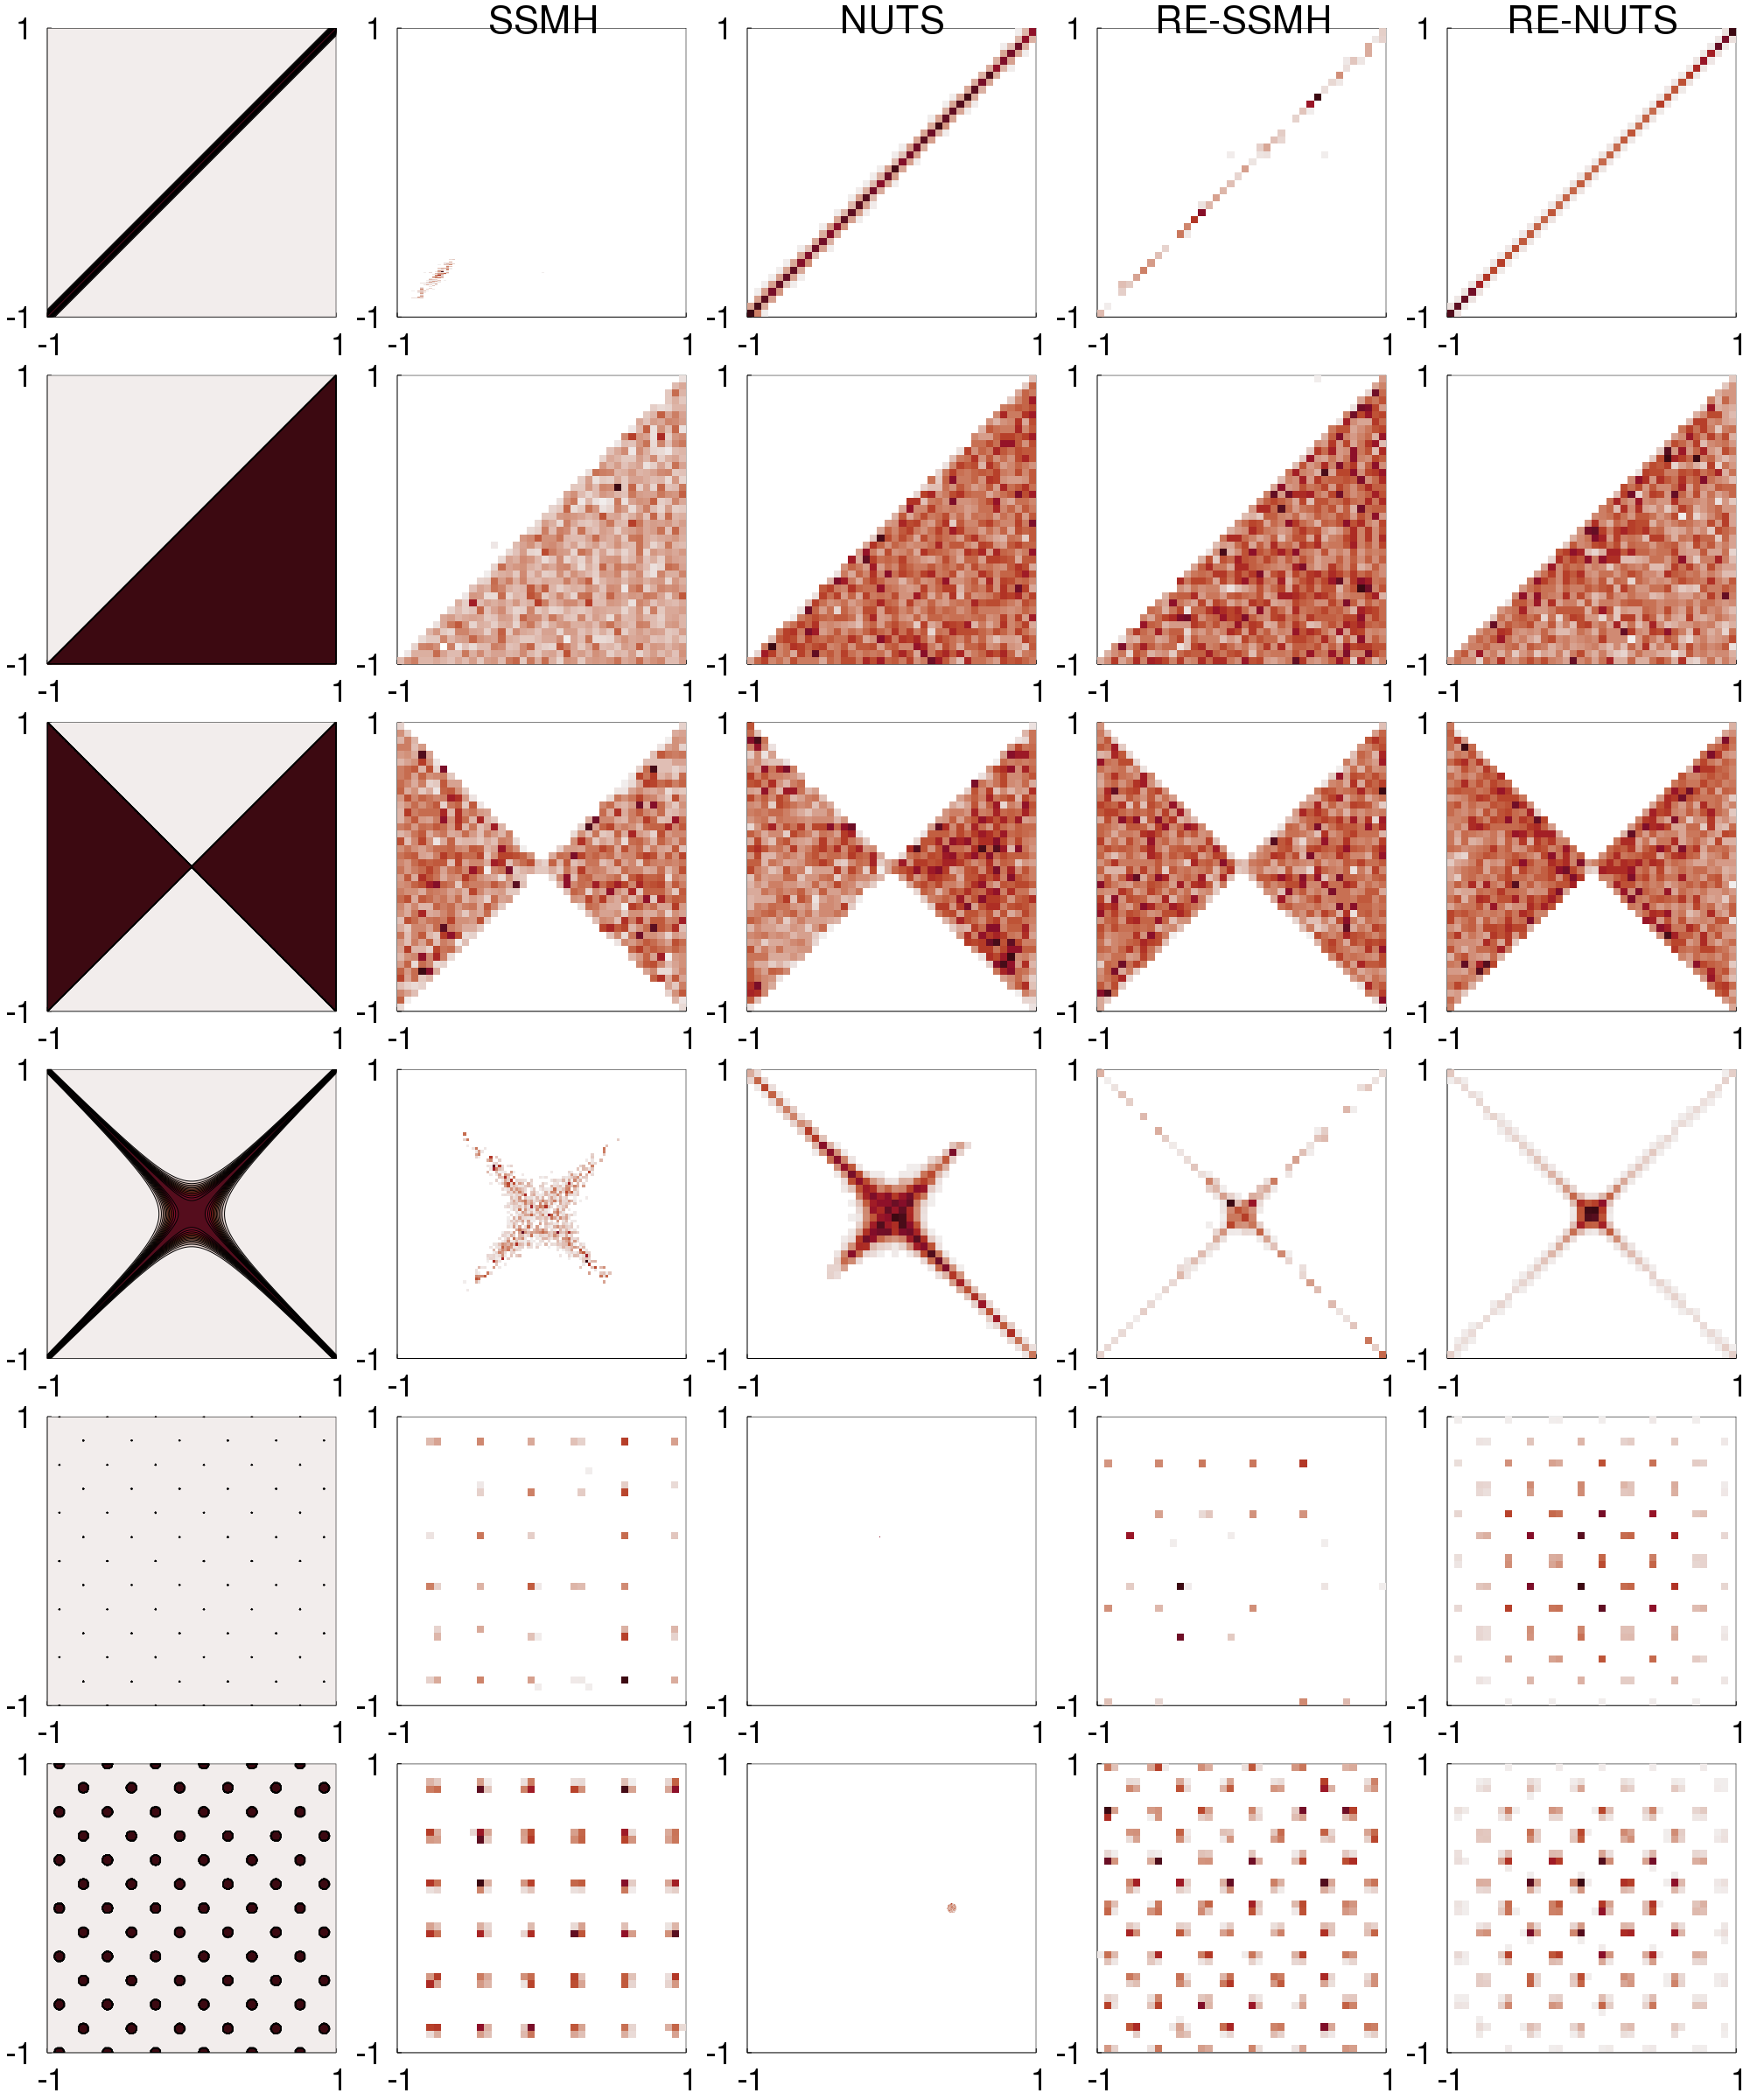
\includegraphics[width=0.9\linewidth,natwidth=2000,natheight=2400]{grid3.png}
% 	\caption{Posterior samples on different problems.  RE: replica exchange, SSMH: Single Site Metropolis Hastings, HMC: Hamiltonian Monte Carlo.  (Left) is target density, and following elements are histograms from computed samples.}
% 	\label{fig:grid}
% \end{figure}
	


\paragraph{Small Models}
In Figure \ref{fig:density} we demonstrate two examples of conditioning on predicates which are non trivial.
First we show that the conditioning can be used to truncate a Gaussian distribution, and the approximation behavior at varying temperatures.  Second we show that two independent random variables can be made equal.  While simple, both are a challenge for probabilistic programming systems because they prevent automatic calculation of the likelihood.

\begin{figure}[!htb]
\centering
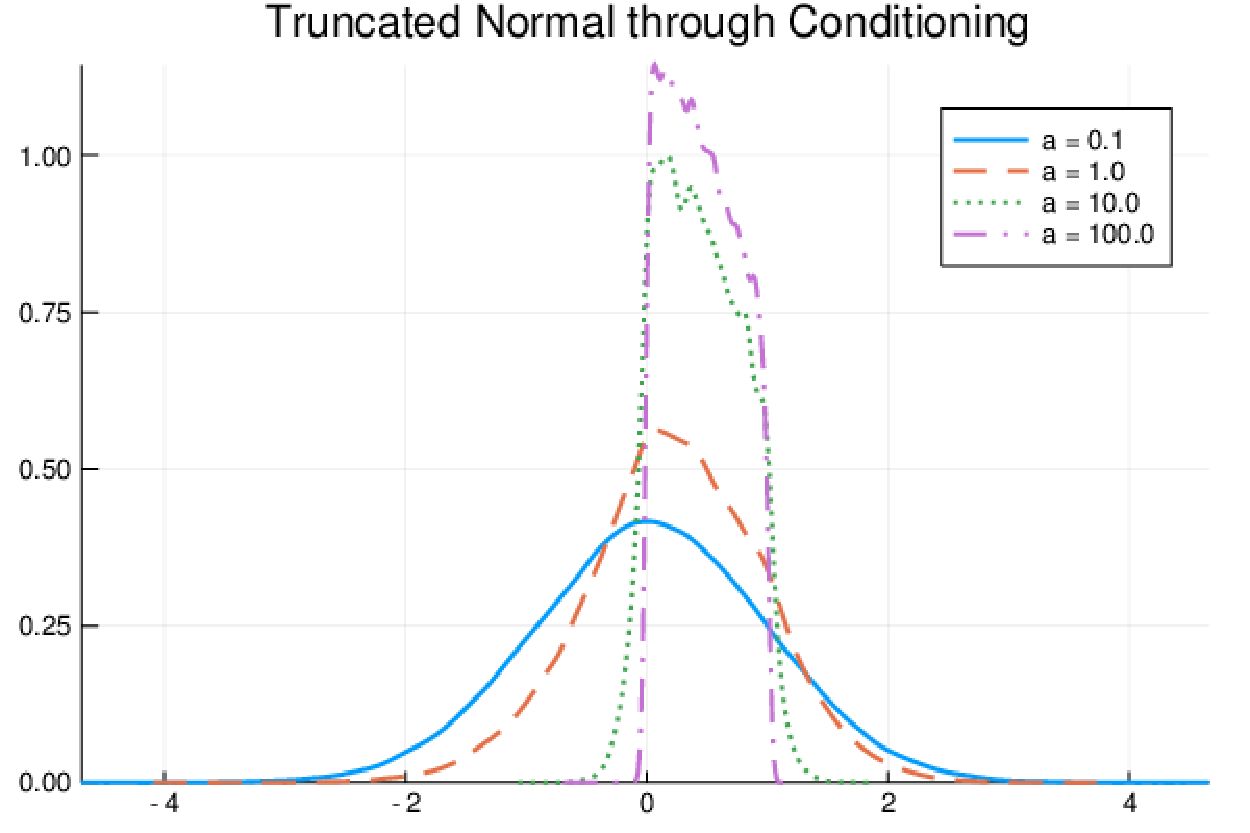
\includegraphics[width=0.8\linewidth]{truncated}

% \begin{minipage}{0.45\linewidth}
% 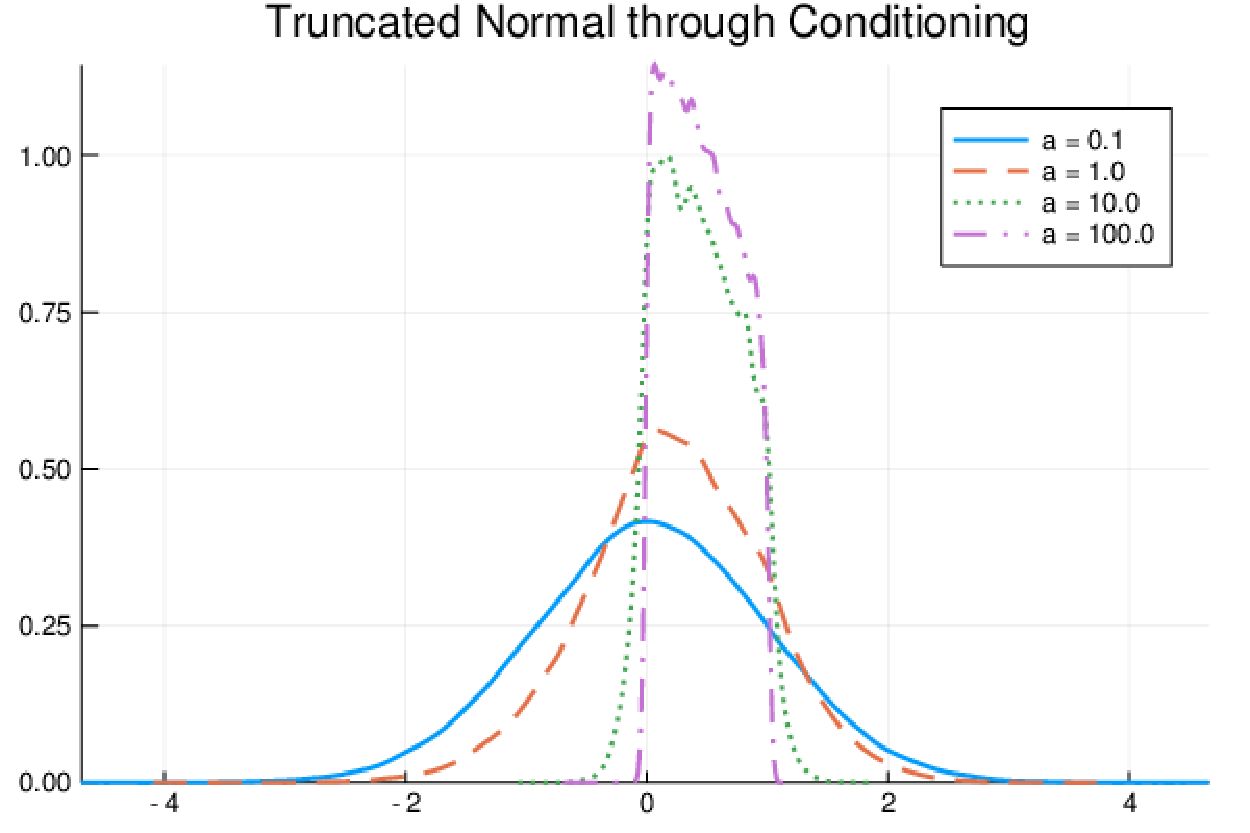
\includegraphics[width=\linewidth]{truncated}
% \end{minipage}%
% \begin{minipage}{0.45\linewidth}
% 	%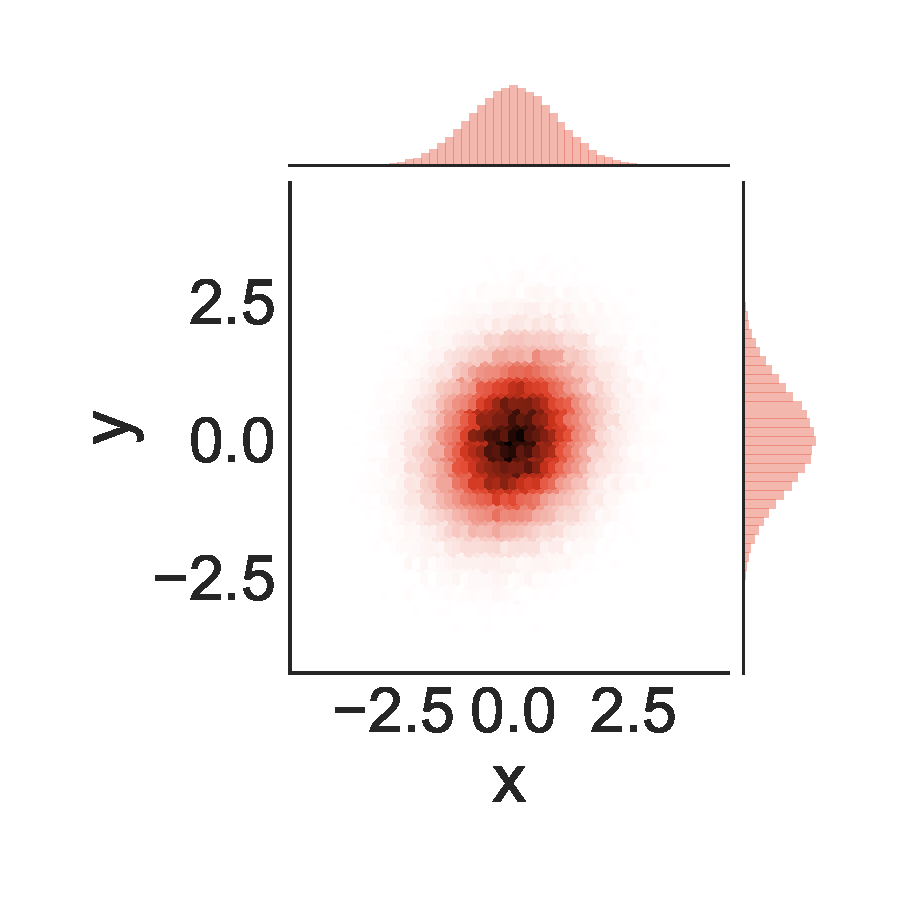
\includegraphics[width=.16\linewidth, trim={1.7cm, 1.6cm, 1.3cm, 1.5cm}, clip]{0-1}
% 	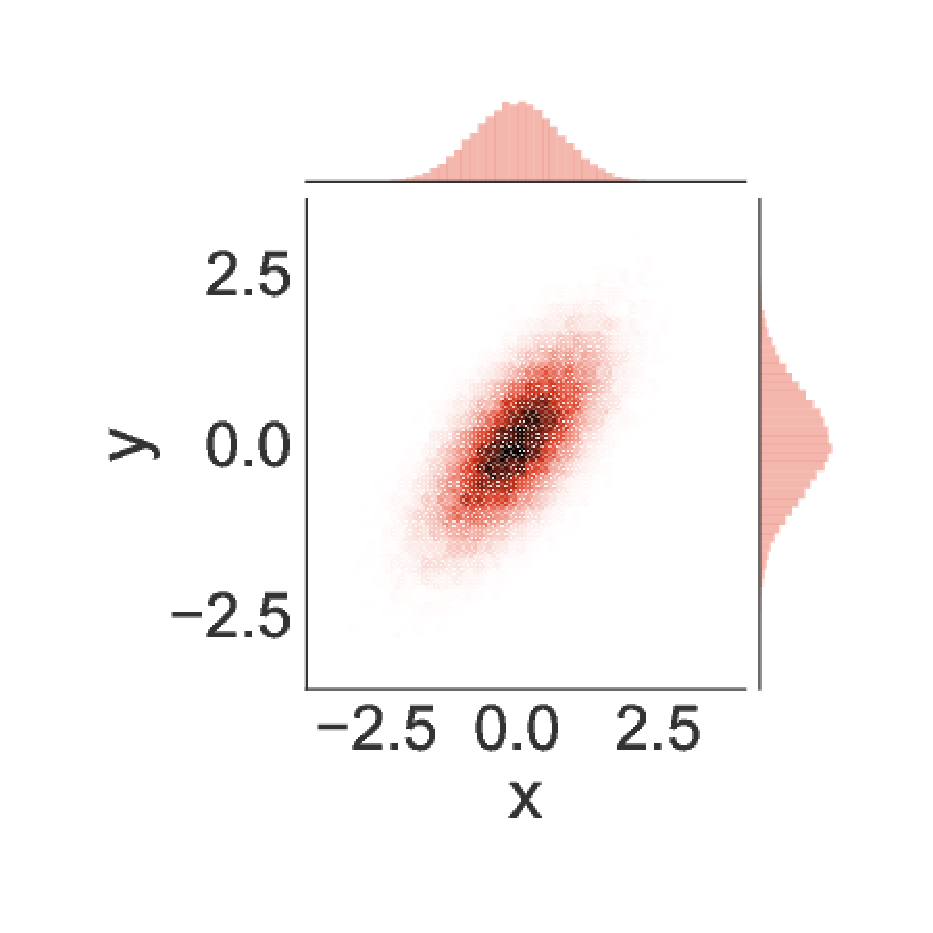
\includegraphics[width=.45\linewidth, trim={1.7cm, 1.6cm, 1.3cm, 1.5cm}, clip]{1-0}
% 	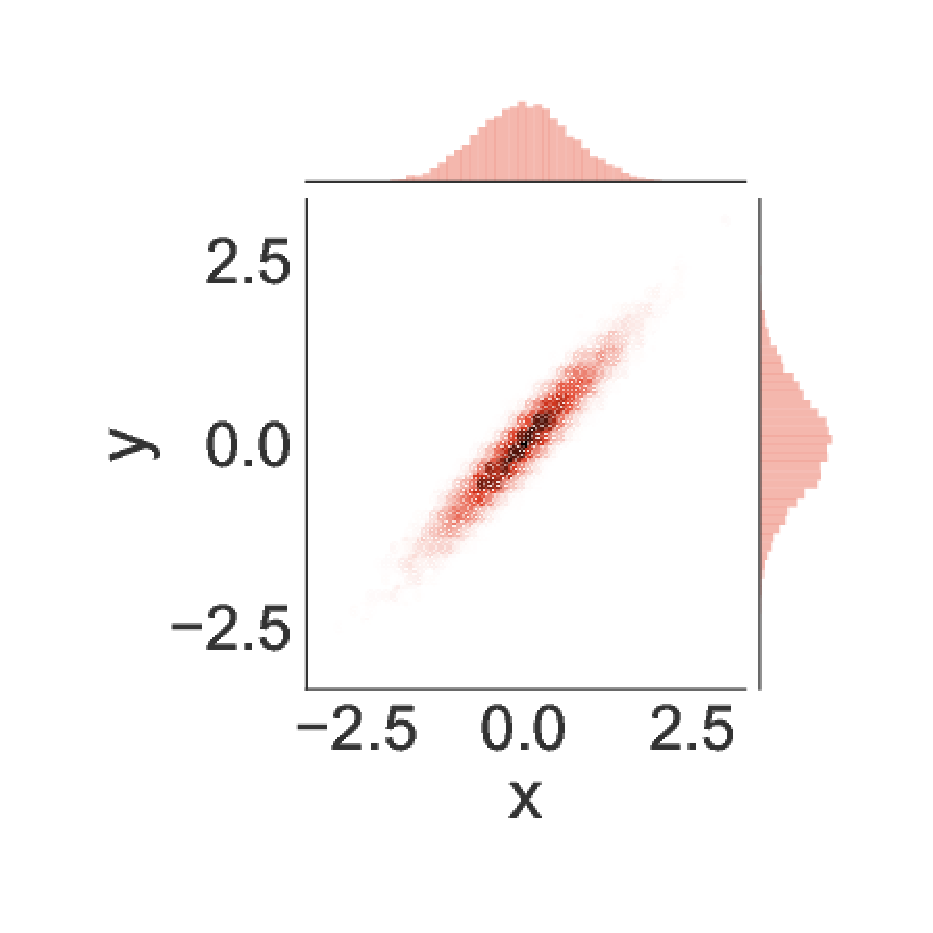
\includegraphics[width=.45\linewidth, trim={1.7cm, 1.6cm, 1.3cm, 1.5cm}, clip]{10-0}
	
% 	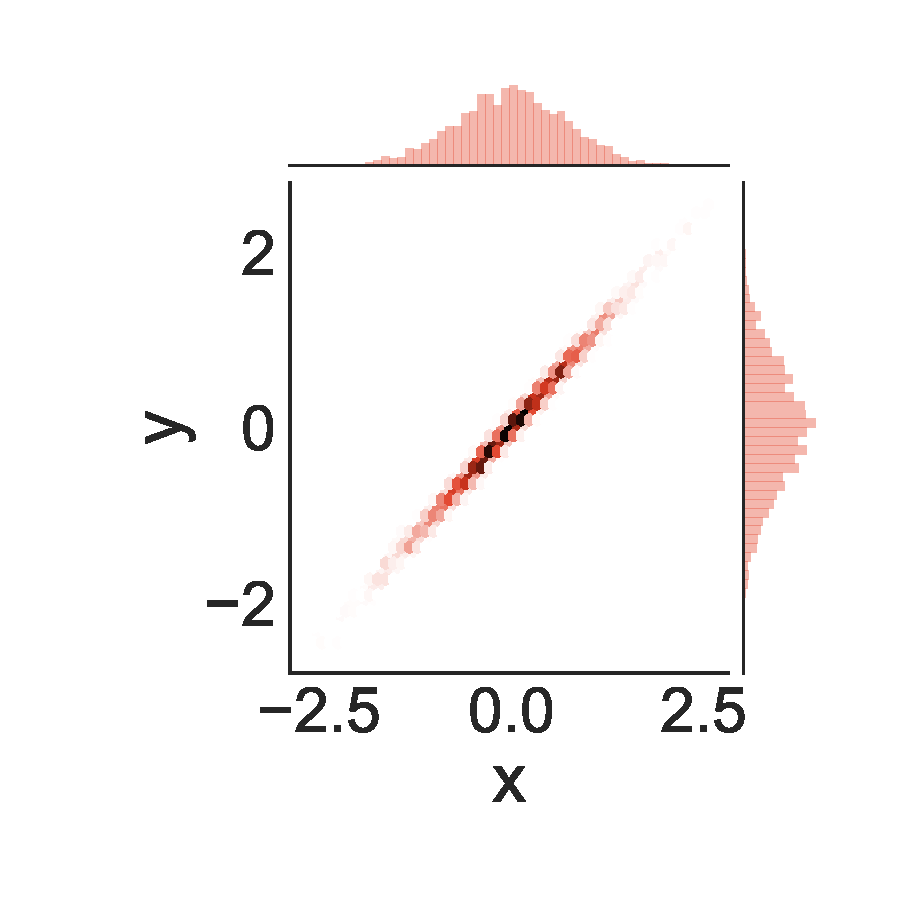
\includegraphics[width=.45\linewidth, trim={1.7cm, 1.6cm, 1.3cm, 1.5cm}, clip]{100-0}
% 	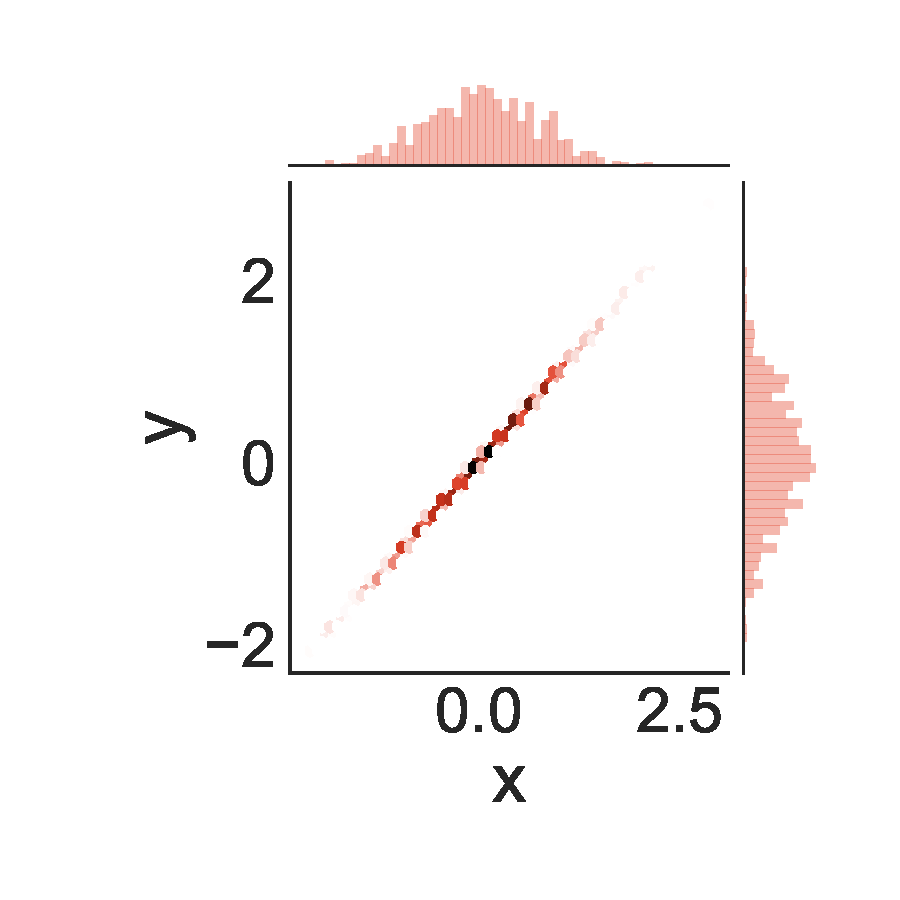
\includegraphics[width=.45\linewidth, trim={1.7cm, 1.6cm, 1.3cm, 1.5cm}, clip]{1000-0}				
	
% %	\fbox{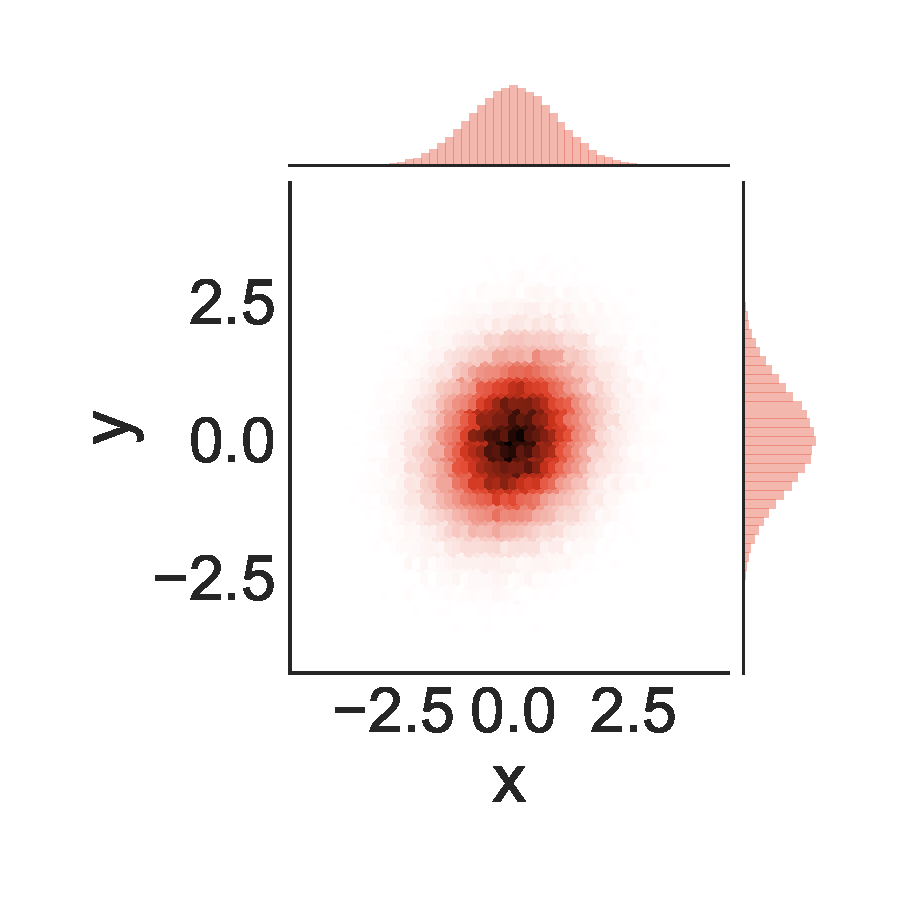
\includegraphics[width=.16\linewidth, trim={1.7cm, 1.6cm, 1.3cm, 1.5cm}, clip]{0-1}}
% %	\fbox{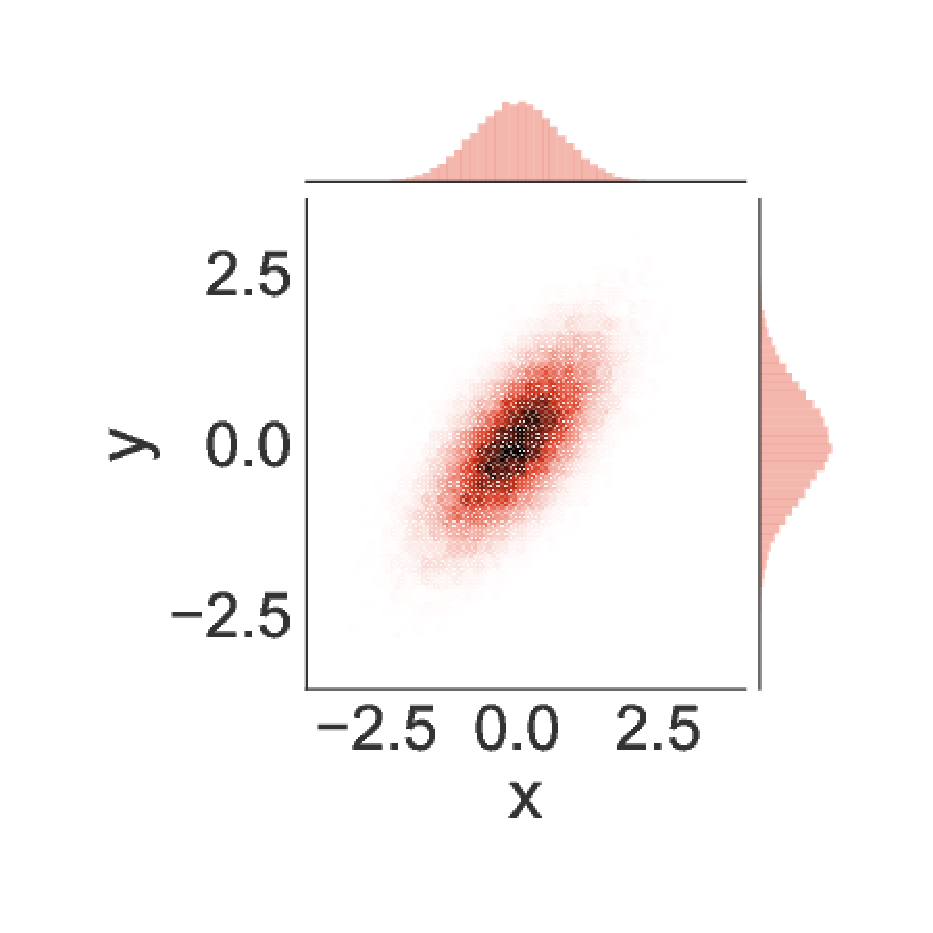
\includegraphics[width=.16\linewidth, trim={1.7cm, 1.6cm, 1.3cm, 1.5cm}, clip]{1-0}}
% %	\fbox{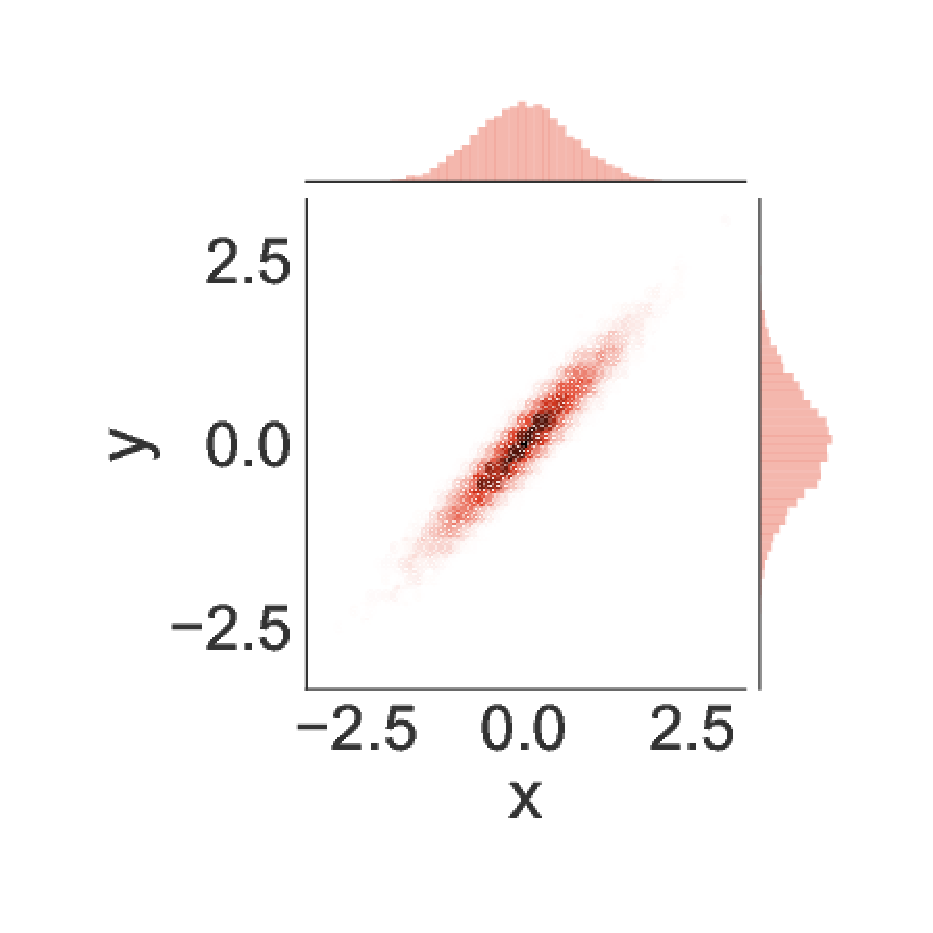
\includegraphics[width=.16\linewidth, trim={1.7cm, 1.6cm, 1.3cm, 1.5cm}, clip]{10-0}}
% %	\fbox{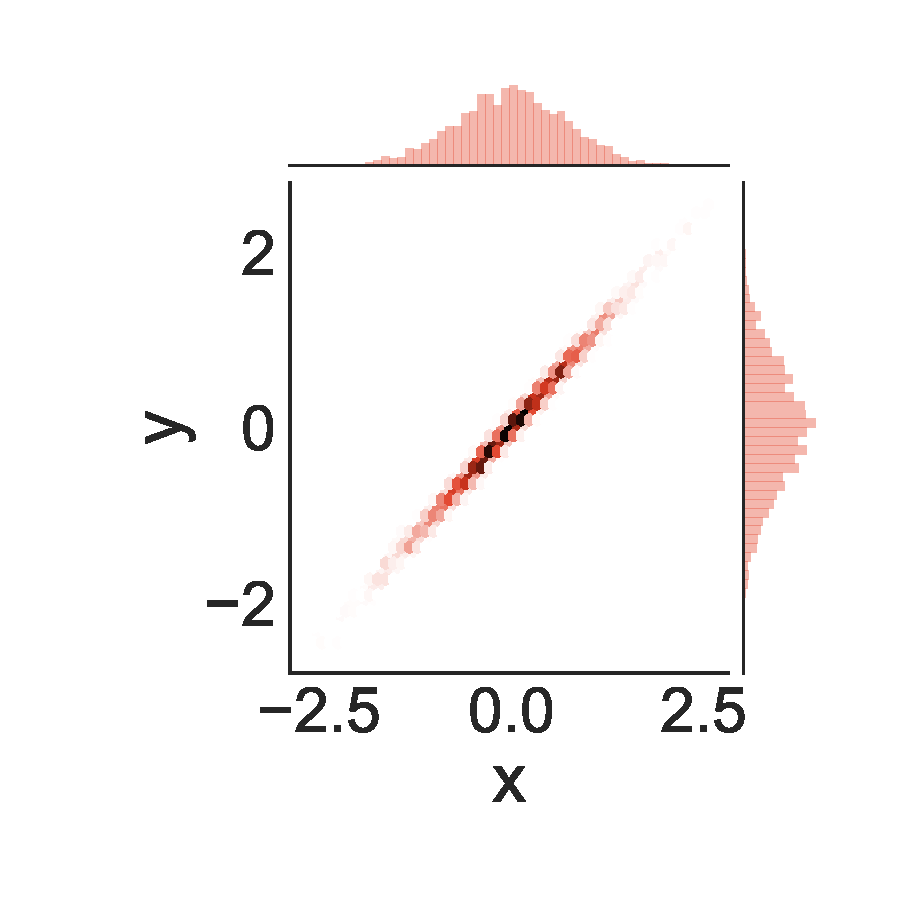
\includegraphics[width=.16\linewidth, trim={1.7cm, 1.6cm, 1.3cm, 1.5cm}, clip]{100-0}}
% %	\fbox{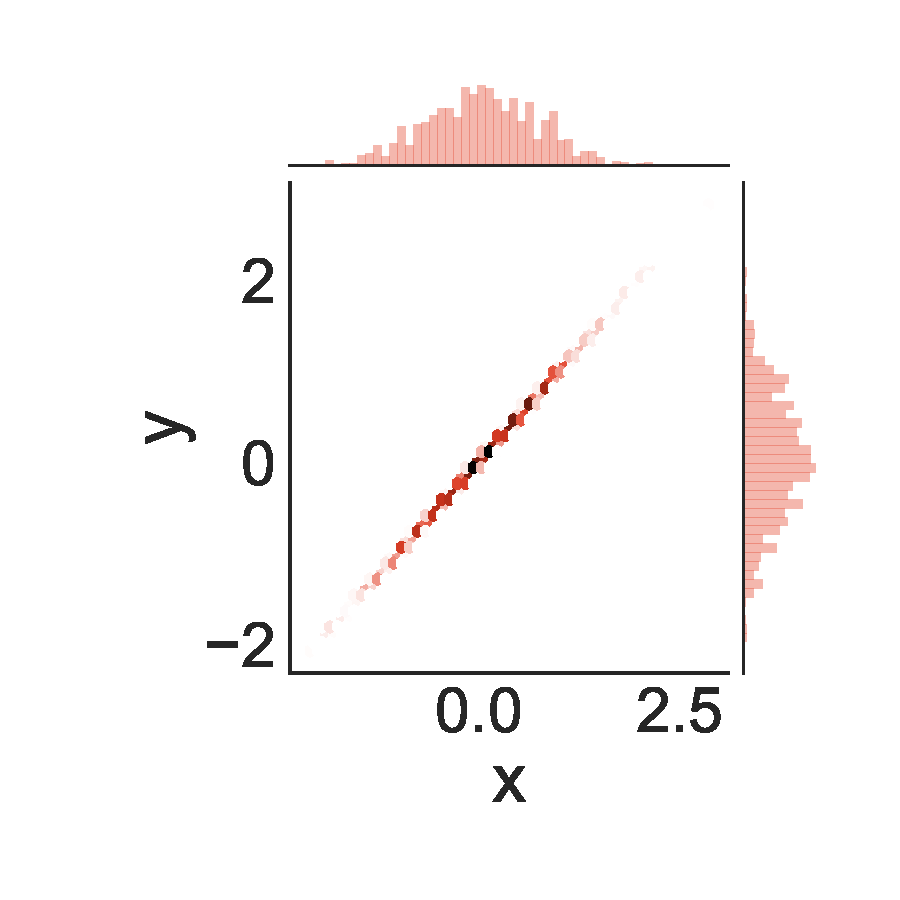
\includegraphics[width=.16\linewidth, trim={1.7cm, 1.6cm, 1.3cm, 1.5cm}, clip]{1000-0}}				
% 	\end{minipage}
	\caption{Left: Density from samples of Gaussian truncated to $[0, 1]$ through conditioning. Right: Conditioning on $X = Y$ where $X$ and $Y$ are independent normal distributions; shown at different temperatures.}
	\label{fig:density}
\end{figure}


\paragraph{Glucose Model}
Type 2 diabetes is a prevalent and costly condition.
Keeping blood glucose within normal limits helps prevent the
long-term complications of Type 2 diabetes like diabetic neuropathy and diabetic retinopathy \citep{brownlee2006glycemic}. Models to predict the trajectories of blood glucose aid in keeping glucose within
normal limits \citep{zeevi2015personalized}. Traditional models have been built from compositions of differential equations \citep{albers2017personalized,levine2017offline} whose parameters are estimated separately for each patient. An alternative approach would be to use a flexible sequence model like an RNN. The problem with this approach is that an RNN can extrapolate to glucose values incompatible with human physiology. This is especially a problem where we have patients with only a few blood glucose measurements. To build an RNN model that respects physiology, we condition on it.

We compare the independent RNN model to the one with declarative knowledge on a second patient from Physionet \citep{moody2001physionet}.
Figure \ref{fig:rnn-samples} plots the results performed on more than 300 pairs of patients.
We see that the conditional model simulates
more realistic glucose dynamics for the patient 
with only a short observed time-series.

% 1) Glucose modeling is a real problem \cite, \cite. 
% 2) Models have focused on ODEs \cite \cite 
% 3) Alternative is to use RNN 
% 4) RNN can produce nonsense result 
% 5) Conditioning helps


% Taken from the supplement in \cite{albers}

% \paragraph{A constrained model of glucose dynamic}
% Take glucose measurements across time $t$ from 
% N patients indexed by $i$: $x_{t,i}$.
% We model the glucose time series for each patient can be modeled independently using a recurrent neural network: 
% \begin{align*}
% W_i &\sim N(0, I) \\
% x_{t, i} &= f(x_{t-1, i}, W).
% \end{align*}
% This model treats all patients as independent. However,
% we have extra knowledge in that the average-across-time glucose levels will be similar across patients. Expressing this kind of knowledge by tying the parameters $W_i, W_j$ is a challenge because the structure of the recurrence function alters how $W$ controls the average outputs. In this sense, we would like to condition on the distance between conditional expectations being close for some distance $d$,
% \begin{align*}
% 	d_E\left(\sum_{t=1}^{T_i} E[x_{t, i} \,|\, W_i], \sum_{t=1}^{T_j} E[x_{t, j} \,|\, W_j]\right) < \delta_E,
% \end{align*}
% for all patient pairs $i, j$. Additionally, we would like to make the series smooth controlling for their variance:
% \begin{align*}
% 	d_{Var}\left(\sum_{t=1}^{T_i} Var[x_{t, i} \,|\, W_i], \sum_{t=1}^{T_j} Var[x_{t, j} \,|\, W_j]\right) < \delta_{Var},
% \end{align*}
%  We compare the independent model
% to the one with the conditional model learned on five patients. 
% We see that the conditional model simulates more realistic glucose dynamics for the patient with only a short observed time-series.

\begin{figure}[!htb]
	\centering
    %\fbox{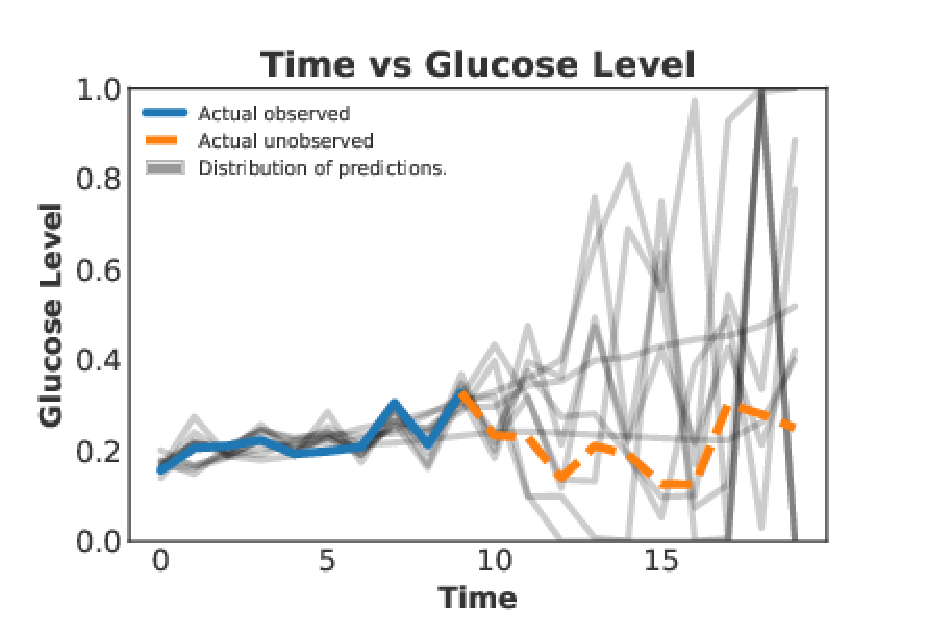
\includegraphics[width=0.30\linewidth, trim={1.cm, 0.1cm, 1.3cm, .5cm}, clip]{rnnsamples-no-tie-py}}
	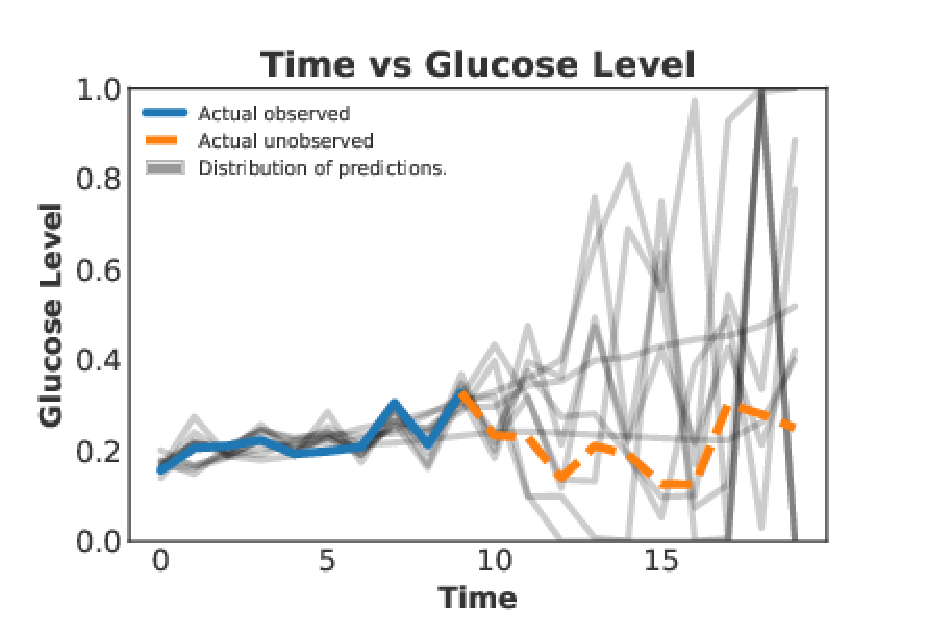
\includegraphics[width=0.45\linewidth, trim={1.cm, 0.1cm, 1.3cm, .5cm}, clip]{rnnsamples-no-tie-py}
	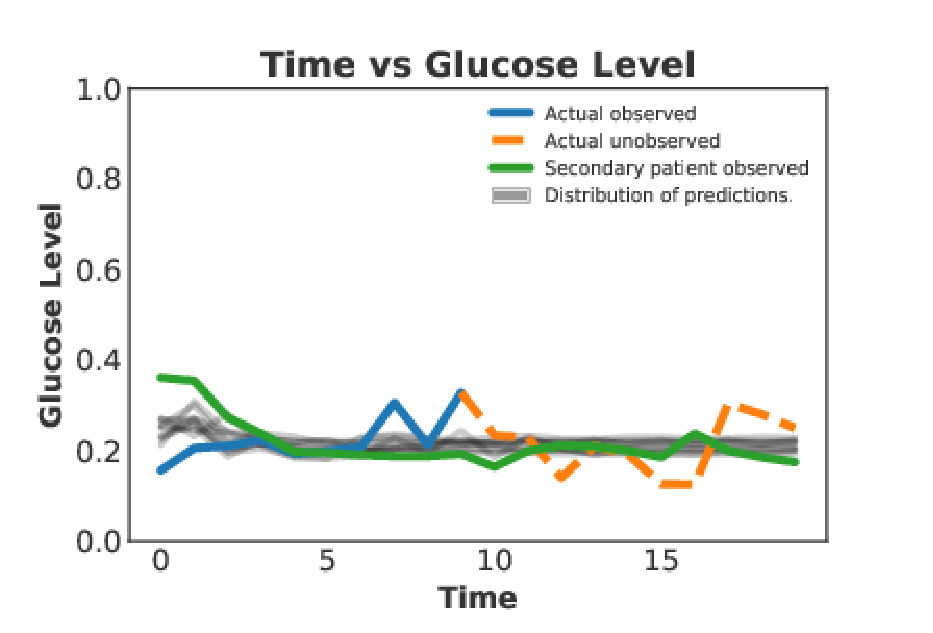
\includegraphics[width=.45\linewidth, trim={1.cm, 0.1cm, 1.3cm, .5cm}, clip]{rnnsamples-py}
	%\fbox{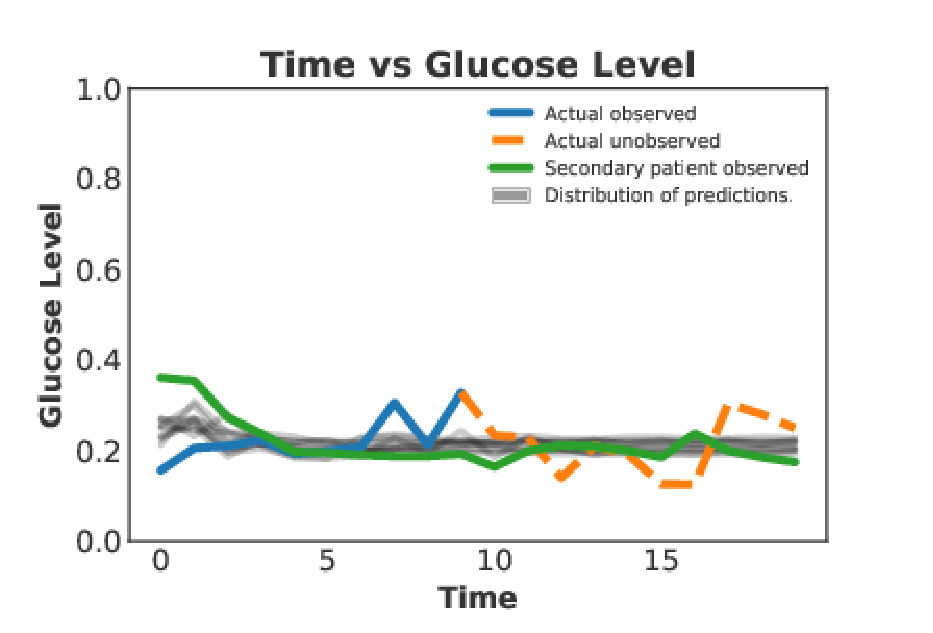
\includegraphics[width=0.30\linewidth, trim={1.cm, 0.1cm, 1.3cm, .5cm}, clip]{rnnsamples-py}}
	%\fbox{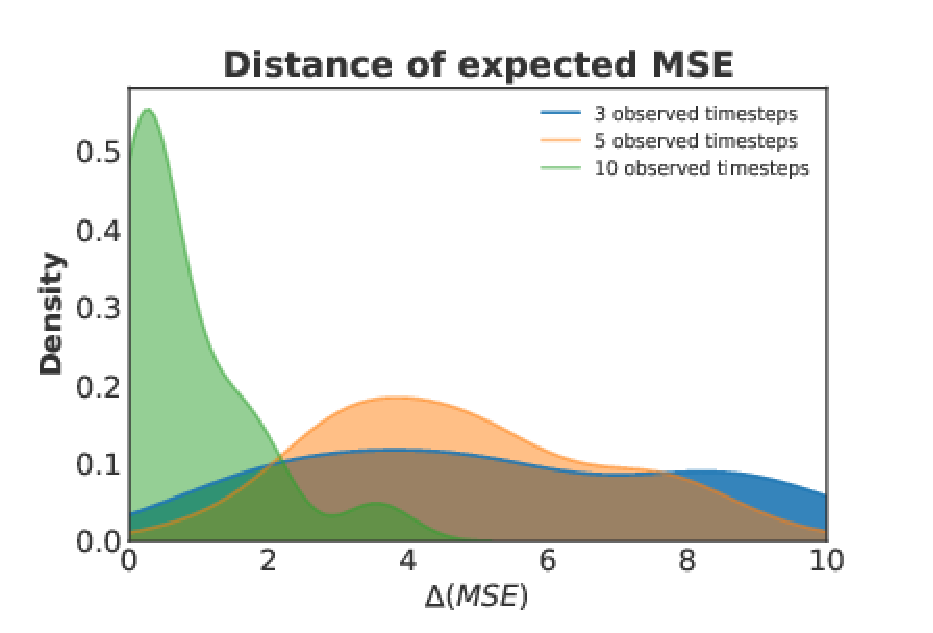
\includegraphics[width=0.30\linewidth, trim={1.cm, 0.0cm, 1.0cm, .5cm}, clip]{delta_mse}}
	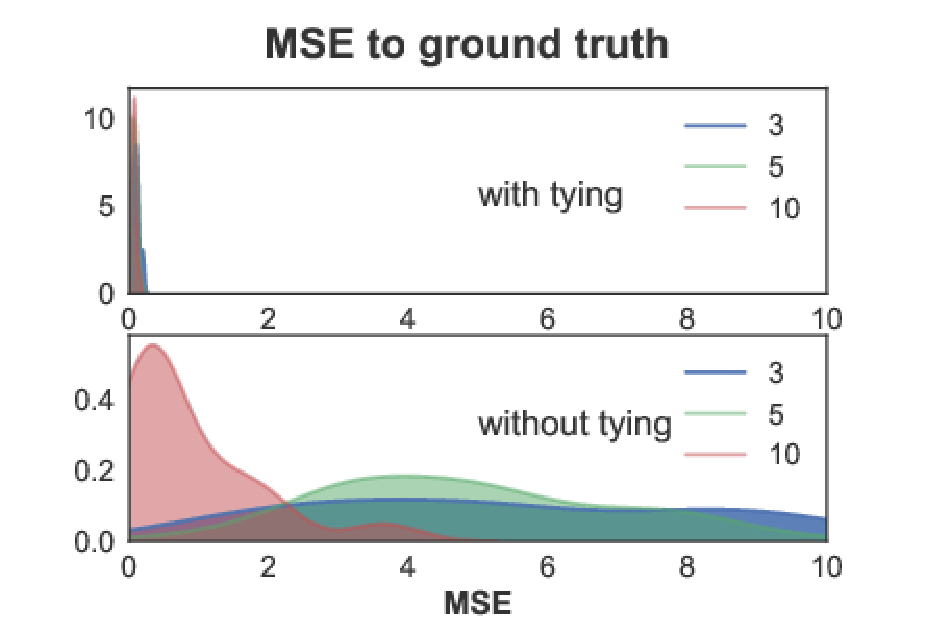
\includegraphics[width=0.9\linewidth, trim={0.7cm, 0.0cm, .7cm, .1cm}, clip]{mse}
		
		\caption{Left: Actual (dotted) and predicted trajectories that were learned using a partial trajectory. Center: Distribution of predicted trajectories learned only using the first ten data points and a tie with a secondary patient. Right, top: MSE when tie is present.  Right, bottom: without tie.  Tying expectations has dramatic influence on prediction error, while as more data is observed, the effect of tying decreases.}
		\label{fig:rnn-samples}
\end{figure}



% Take the same glucose measurements from 5 patients. Make a probabilistic RNN with
% independent parameters for each patient. Then add the constraint that the means are
% close. Then look at the prediction for one patient where we remove all but the
% first few time steps and show the forward predictions are better with the added knowledge
% that the means are close across patients.


% \paragraph{Transfer Learning}
% In transfer learning, we hope to use information from one learning problem to
% help with another learning problem. One way this has been accomplished in
% deep learning is to use
% the parameters of a model learned in one domain as the initialization for the
% parameters in a another domain. We could accomplish a similar thing via conditioning
% by having the weights of both models be close. But with conditioning, this is not
% the only choice, we can have the first layer activations be close in distribution
% in both the source and target transfer domain. Concretely, consider the following
% two layer stochastic neural network for each domain where the $i$th covariate
% label pair $(x_i, y_i)$ is
% \begin{align*}
% W \sim p(W)
% z_{2, i} &\sim p(z_{2, i} | x_i, W_2) \\
% z_{1, i} &\sim p(z_{1, i} | z_{2, i}, W_1) \\
% y_{i} &\sim p(y_i | z_{1, i})
% \end{align*}


% \section{Related Work}
% \begin{itemize}

% \item Existing Notion of Probablistic Programs
% Probabilistic programming languages and the inference algorithms which support them differ primarily in how probability distributions are represented.
% % In this contribution we define the sample space as an $n$-dimensional unit hypercube
% % $\Omega = [0, 1]^n$, and by $(\omega_1,...,\omega_n)$ denote an element of $\Omega$.
% % In addition, we define $\mu$ as the Lebesgue measure.
% % Random variables are transformations of $\Omega$, and act on some or all of its dimensions.
% % For example a random variable $\mathcal{U}_{a,b}: \Omega \to \mathbb{R}$, which is distributed uniformly between $a$ and $b$ could be defined simply as:
% % $$
% % \mathcal{U}_{a,b}(\omega) = a + \omega_1(b - a)
% % $$
% \item Make explicit how the measure theortic formulation connects to the sampling process
% \end{itemize}
